Neste capítulo, exploramos a hipótese de que a formação de câmaras de eco em uma rede social pode ser matematicamente representada através de uma combinação de várias estatísticas descritivas, cada uma correspondendo a um critério específico para a detecção de câmaras de eco. Esses critérios incluem a densidade da comunidade, a homogeneidade das opiniões, as conexões externas e o efeito de influenciadores, todos fundamentais para entender a dinâmica das redes sociais e, mais especificamente, a formação de câmaras de eco. Através da análise detalhada de cada critério e da introdução de parâmetros adicionais como o Coeficiente Individual de Câmara de Eco (ECC) e o Parâmetro Global de Câmara de Eco (GEC), buscamos desenvolver um modelo matemático que possa quantificar a probabilidade de formação de câmaras de eco em uma rede social. Este modelo é posteriormente implementado computacionalmente através da classe Python EchoChamberDetector, que utiliza algoritmos consagrados para identificação de comunidades e análise de redes sociais. A implementação permite não apenas a identificação de potenciais câmaras de eco, mas também oferece insights sobre a influência de diferentes fatores na sua formação, proporcionando uma ferramenta robusta e adaptável para análise de redes sociais no contexto da detecção de câmaras de eco.

\section{Heurísticas para detecção Câmaras de Eco}

Nossa hipótese é que a probabilidade de formação de câmaras de eco em uma rede social pode ser expressa matematicamente como uma combinação de várias estatísticas descritivas, cada uma correspondendo a um critério específico para a detecção de câmaras de eco:

\begin{itemize}
	\item \textbf{Densidade da comunidade}: A densidade da comunidade é uma medida do grau de interconexão entre os membros de uma comunidade. Em uma rede social, podemos calcular a densidade da comunidade como a proporção de conexões possíveis que realmente existem entre os membros da comunidade. Uma comunidade densa é aquela em que os membros estão altamente interconectados. Em termos de redes sociais, isso pode ser medido pelo número de conexões que cada indivíduo tem dentro de sua comunidade. Uma comunidade densa é mais propensa a formar uma câmara de eco, pois a informação circula predominantemente dentro do grupo, reforçando as opiniões existentes \cite{2015_Recuero_BOOK}.

	\item \textbf{Homogeneidade das opiniões}: A homogeneidade das opiniões refere-se ao grau de concordância ou semelhança nas opiniões dos membros de uma comunidade. Em uma rede social, isso pode ser medido pela frequência com que certas opiniões ou pontos de vista são compartilhados ou endossados pelos membros da comunidade. Quanto mais homogêneas forem as opiniões dentro de uma comunidade, maior será a probabilidade de uma câmara de eco se formar \cite{2016_WanYu}.

	\item \textbf{Conexões externas}: As conexões externas referem-se às interações entre os membros de uma comunidade e indivíduos ou grupos fora da comunidade. Em uma rede social, isso pode ser medido pelo número de conexões que cada indivíduo tem fora de sua comunidade. Quanto menor o número de conexões externas, maior a probabilidade de câmaras de eco se formarem, pois a informação é menos provável de ser desafiada por opiniões divergentes \cite{ref3}.

	\item \textbf{Efeito de influenciadores}: Os influenciadores são indivíduos ou grupos que têm um impacto significativo sobre as opiniões e comportamentos dos outros em uma rede social. Em uma rede social, isso pode ser medido pela centralidade do nó, ou seja, o número de conexões que um indivíduo tem, ou pelo número de vezes que o conteúdo de um indivíduo é compartilhado ou endossado por outros. A presença de influenciadores na rede pode influenciar a formação de câmaras de eco, pois eles podem reforçar opiniões existentes e promover a homogeneidade dentro da comunidade \cite{2014_Gilbuena}.
\end{itemize}

Antes de mergulharmos na formulação matemática, é crucial entender e definir claramente o que constitui uma "câmara de eco". Em contextos de redes sociais, uma câmara de eco é frequentemente vista como um ambiente em que os indivíduos são expostos predominantemente a informações que reforçam suas crenças e opiniões preexistentes, limitando assim a exposição a perspectivas divergentes. Este fenômeno pode resultar em polarização de opiniões e uma percepção distorcida da realidade. Além disso, ao considerar a metodologia proposta por Atiqi, é essencial destacar a relevância dos parâmetros GEC (Global Echo Chamber) e ECC (Individual Echo Chamber Coefficient). Enquanto o GEC fornece uma visão macro da tendência da rede inteira em formar câmaras de eco, o ECC se concentra na propensão individual de cada membro da rede em se isolar em tais câmaras. A inclusão desses parâmetros oferece uma abordagem mais holística, permitindo uma análise tanto no nível da rede como um todo quanto no nível individual.

No contexto da plataforma Colab, uma 'câmara de eco' pode ser definida como \textit{um subconjunto de usuários que, ao interagir predominantemente com tópicos específicos de zeladoria pública (como bueiros, poda de árvores, segurança, falta de luz, entre outros), demonstram uma homogeneidade notável em suas opiniões e perspectivas.} Esta homogeneidade é quantificada através da métrica de 'homogeneidade de opiniões', enquanto a 'average exposure' refere-se à frequência média com que um usuário é exposto a opiniões alinhadas às suas próprias crenças dentro desses tópicos. Em essência, uma câmara de eco no Colab indica uma tendência de agrupamento de usuários que compartilham e reforçam visões semelhantes, limitando assim a diversidade de perspectivas a que são expostos.

Com base nessas hipóteses e definiçõess, podemos construir um modelo que inclua essas estatísticas descritivas. O modelo será usado para estimar os parâmetros que quantificam a influência dessas estatísticas na probabilidade de formação de câmaras de eco. Podemos expressar a probabilidade de formação de câmaras de eco como uma função de várias estatísticas descritivas:

\begin{equation}
	\begin{split}
		P(\text{{EchoChamber}}) = \exp(&\beta_1 \cdot \text{{CommunityDensity}} + \\
		&\beta_2 \cdot \text{{HomogeneityOfOpinions}} + \\
		&\beta_3 \cdot \text{{ExternalConnections}} + \\
		&\beta_4 \cdot \text{{Influencers}} + \\
		&\beta_5 \cdot \text{{AverageExposure}} + \\
		&\beta_6 \cdot \text{{GEC}} + \\
		&\beta_7 \cdot \text{{ECC}})
	\end{split}
\end{equation}

em que $\beta_1$, $\beta_2$, $\beta_3$, $\beta_4$, $\beta_5$, $\beta_6$ e $\beta_7$ são os parâmetros estimados para cada estatística descritiva e exp é a função exponencial. Essa equação fornece uma maneira de quantificar matematicamente a probabilidade de formação de câmaras de eco em uma rede social, com base nos critérios estabelecidos. Os parâmetros $\beta$ são comumente usados para quantificar a influência de várias estatísticas descritivas na probabilidade de formação de eventos complexos. Os valores dos parâmetros $\beta$ são geralmente estimados a partir dos dados. No entanto, a escolha dos valores iniciais para esses parâmetros pode ter um impacto significativo na convergência do modelo. Portanto, é comum iniciar os parâmetros beta com valores simples, como 1, e ajustá-los iterativamente para melhorar o ajuste do modelo.

Os parâmetros beta podem ser interpretados em termos de suas implicações para a probabilidade de formação de câmaras de eco. Por exemplo, um valor positivo para o parâmetro beta associado à densidade da comunidade sugeriria que comunidades mais densas têm maior probabilidade de formar câmaras de eco. Analogamente, um valor positivo para o parâmetro beta associado à homogeneidade das opiniões indicaria que comunidades com opiniões mais homogêneas têm maior probabilidade de formar câmaras de eco. Os aspectos de escala a serem considerados dependem dos critérios específicos empregados para detectar câmaras de eco. Por exemplo, ao considerar a densidade da comunidade como um critério, a escala pode ser considerada em termos do número de conexões dentro da comunidade em relação ao número total de conexões possíveis. Se a homogeneidade das opiniões for um critério, a escala pode ser considerada em termos da variação das opiniões dentro da comunidade.

\subsection{Implementação Computacional do Teorema de Probabilidade de Câmaras de Eco}

Para aplicar nosso teorema de probabilidade de câmaras de eco na prática, desenvolvemos a classe Python EchoChamberDetector implementada em \autoref{codigo:echochamberdetector}. Essa classe permite analisar redes sociais e identificar potenciais câmaras de eco com base nos critérios estabelecidos em nosso teorema.

A classe EchoChamberDetector utiliza dois algoritmos diferentes, Louvain e Girvan-Newman, para identificar comunidades dentro da rede social. Esses algoritmos são usados como etapas preliminares para posterior análise e identificação de câmaras de eco. O algoritmo de Louvain é um método popular para detecção de comunidades em redes sociais. Ele se baseia na otimização da modularidade da rede, buscando agrupar nós que estejam mais densamente conectados entre si do que com o restante da rede. O algoritmo de Louvain é eficiente e adequado para identificar comunidades sobrepostas. Já o algoritmo de Girvan-Newman é baseado na ideia de remover sucessivamente as arestas de maior betweenness centrality da rede, dividindo-a em comunidades menores. Esse processo é repetido até que todas as arestas sejam removidas e as comunidades sejam completamente separadas. O algoritmo de Girvan-Newman é mais lento do que o de Louvain, mas é capaz de identificar comunidades hierárquicas e não sobrepostas.

Uma vez que as comunidades foram identificadas usando um dos algoritmos, prosseguimos com a análise das câmaras de eco. Para cada comunidade detectada, realizamos cálculos estabelecendo relações entre a comunidade da rede com o resto da rede como um todo:

\begin{itemize}
	\item Fator de densidade da comunidade: calculado usando a função \texttt{calculate\_community\_density}, que mede a proporção de arestas existentes em relação ao número máximo possível de arestas na comunidade. Quanto maior a densidade, maior a probabilidade de formação de uma câmara de eco.
	\item Homogeneidade das opiniões: calculada usando a função \texttt{calculate\_homogeneity\_of\_opinions}, que calcula o desvio padrão das pontuações de opiniões dos membros da comunidade. Quanto menor o desvio padrão, maior a homogeneidade das opiniões e maior a probabilidade de formação de uma câmara de eco.
	\item Fator de conexões externas: calculado usando a função \texttt{calculate\_external\_connections}, que mede a proporção de conexões da comunidade que são externas, ou seja, que se conectam a nós fora da comunidade. Quanto menor o número de conexões externas, maior a probabilidade de formação de uma câmara de eco.
	\item Fator de influenciadores: calculado usando a função \texttt{calculate\_influencers}, que calcula a proporção de influenciadores presentes na comunidade em relação ao tamanho total da comunidade. Quanto maior a proporção de influenciadores, maior a probabilidade de formação de uma câmara de eco.
\end{itemize}

Além dessas estatísticas, também incorporamos duas heurísticas adicionais baseadas no trabalho de \citeonline{2023_Atiqi_BOOK}: Parâmetro Global de Câmara de Eco (GEC) e Exposição média.

A metodologia de cálculo do Parâmetro Global de Câmara de Eco (GEC) é baseada na abordagem apresentada por \citeonline{2023_Atiqi_BOOK}. O GEC é uma medida da tendência geral de uma rede social para formar câmaras de eco. Ele é calculado como a soma do produto dos sinais das opiniões de todos os pares de usuários conectados na rede.

Para calcular o GEC, primeiro precisamos definir a opinião de um usuário. No contexto de redes sociais, a opinião de um usuário é geralmente representada por um score que reflete a polaridade de suas postagens ou interações. Valores mais próximos de 1 representam postagens mais positivas, enquanto valores mais próximos de 0 representam sentimentos mais negativos.

Dado um par de usuários conectados $(u, v)$, o produto dos sinais de suas opiniões é dado por $\text{sign}(o_u) \cdot \text{sign}(o_v)$, onde $o_u$ e $o_v$ são as opiniões dos usuários $u$ e $v$, respectivamente, e $\text{sign}$ é a função sinal que retorna -1 para números negativos, 0 para zero e 1 para números positivos.

O GEC é então calculado somando o produto dos sinais das opiniões de todos os pares de usuários conectados na rede:

\begin{equation}
	GEC = \sum_{(u, v) \in E} \text{sign}(o_u) \cdot \text{sign}(o_v)
\end{equation}

em que $E$ é o conjunto de todas as arestas na rede.

Um valor positivo de GEC indica uma tendência para a formação de câmaras de eco, pois sugere que os usuários tendem a se conectar com outros usuários que compartilham opiniões semelhantes. Por outro lado, um valor negativo de GEC indica uma tendência para a diversidade de opiniões, pois sugere que os usuários tendem a se conectar com outros usuários que têm opiniões diferentes.

É importante notar que o GEC é uma medida global que reflete a tendência geral da rede para formar câmaras de eco. Ele não fornece informações sobre a formação de câmaras de eco em nível de comunidade ou individual. Para obter essas informações, precisamos de outras medidas ou heurísticas, como as discutidas na seção anterior.

A exposição média é outra heurística importante que Atiqi introduz em sua metodologia. Definida como a soma das diferenças entre a opinião do usuário e o sentimento da notícia exposta, média sobre todos os usuários. Matematicamente, isso pode ser expresso como:

\begin{equation}
	\text{{Exposição Média}} = \frac{1}{N} \sum_{i=1}^{N} |o_i - s_j|
\end{equation}

em que $o_i$ é a opinião do usuário $i$, $s_j$ é o sentimento da notícia $j$ exposta ao usuário $i$, e $N$ é o número total de usuários na rede.

A exposição média é uma medida de quão expostos os usuários estão a opiniões que diferem das suas. Uma alta exposição média indica que os usuários estão sendo expostos a uma variedade de opiniões, o que pode reduzir a probabilidade de formação de câmaras de eco. Por outro lado, uma baixa exposição média sugere que os usuários estão principalmente expostos a opiniões que são semelhantes às suas, aumentando a probabilidade de formação de câmaras de eco.

No contexto do Colab, a exposição média pode ser calculada aproveitando os tipos de postagens com os quais os usuários mais interagem. Cada tipo de evento, seja ele relacionado a infraestrutura, segurança pública, entre outros, pode ser representado como um número único. Isso cria um vetor de características para cada usuário que reflete os tipos de eventos com os quais ele interage. A exposição média de um usuário pode então ser calculada como a diferença entre o vetor de características do usuário e o vetor médio de características de todos os eventos na rede.

Matematicamente, isso pode ser expresso da seguinte maneira:

\begin{equation}
	\text{{Exposição Média}} = \frac{1}{N} \sum_{i=1}^{N} ||v_i - \bar{v}||
\end{equation}

em que $v_i$ é o vetor de características do usuário $i$, $\bar{v}$ é o vetor médio de características de todos os eventos na rede, e $N$ é o número total de usuários na rede. A norma $||.||$ pode ser a norma euclidiana, que mede a distância geométrica entre os dois vetores, ou outra norma apropriada.

Nesse contexto, um usuário que interage com uma variedade de tipos de eventos terá uma exposição média menor, pois seu vetor de características será mais semelhante ao vetor médio de características de todos os eventos. Por outro lado, um usuário que interage principalmente com um tipo específico de evento terá uma exposição média maior, pois seu vetor de características será mais diferente do vetor médio.

Essa abordagem permite uma análise mais granular da exposição dos usuários a diferentes tipos de eventos e pode ajudar a identificar usuários ou comunidades que estão potencialmente isolados em câmaras de eco.

\begin{itemize}
	\item \textbf{Exposição média}: A exposição média é definida como a soma das diferenças entre a opinião do usuário e o sentimento das notícias expostas, média sobre todos os usuários. Isso é calculado usando a função \texttt{calculate\_average\_exposure}. Quanto maior a exposição média, maior a probabilidade de formação de uma câmara de eco, pois indica que os usuários estão sendo expostos a notícias que reforçam suas opiniões existentes.
	\item \textbf{Parâmetro Global de Câmara de Eco (GEC)}: O GEC é definido como a soma do produto dos sinais das opiniões de todos os pares de usuários conectados na rede. Isso é calculado usando a função \texttt{calculate\_gec}. Um valor positivo de GEC indica uma tendência para a formação de câmaras de eco, pois sugere que os usuários tendem a se conectar com outros usuários que compartilham opiniões semelhantes.
\end{itemize}

Com base nessas estatísticas, a probabilidade de formação de câmaras de eco é calculada usando a função \texttt{calculate\_echo\_chamber\_probability}. Esta função calcula a probabilidade como uma função exponencial das estatísticas descritivas, ponderadas pelos parâmetros beta correspondentes. A comunidade é então classificada como uma câmara de eco se a sua probabilidade de formação de câmara de eco for maior ou igual à probabilidade de formação de câmara de eco para toda a rede.

A função \texttt{is\_echo\_chamber} em nossa implementação Python exemplifica a aplicação conjunta de medidas globais e locais na detecção de câmaras de eco. A função calcula a probabilidade de formação de câmaras de eco tanto na rede inteira quanto em uma comunidade específica. A probabilidade global é calculada pela linha \texttt{graph\_probability = self.calculate\_echo\_chamber\_probability(list(self.G.nodes))}, que considera todas as conexões e opiniões na rede, semelhante ao GEC. Por outro lado, a probabilidade local é calculada pela linha \texttt{community\_probability = self.calculate\_echo\_chamber\_probability(community)}, que considera apenas as conexões e opiniões dentro da comunidade.

A comparação \texttt{community\_probability >= graph\_probability} é então usada para determinar se a comunidade é uma câmara de eco. Se a probabilidade de formação de câmaras de eco na comunidade for maior ou igual à probabilidade na rede como um todo, a função retorna \texttt{True}, indicando que a comunidade é uma câmara de eco.

Essa abordagem ilustra a importância de combinar medidas globais e locais na detecção de câmaras de eco. Enquanto medidas globais como o GEC fornecem uma visão geral da tendência da rede para formar câmaras de eco, medidas locais são necessárias para identificar câmaras de eco específicas e entender a dinâmica dentro dessas comunidades.

A classe EchoChamberDetector fornece uma implementação computacional do nosso teorema de probabilidade de câmaras de eco, permitindo a identificação de potenciais câmaras de eco em redes sociais. No entanto, é importante notar que a detecção de câmaras de eco é um problema complexo que pode não ser totalmente capturado por qualquer conjunto de heurísticas. Portanto, é sempre uma boa ideia testar essas heurísticas em uma variedade de dados e contextos para ver como elas se comportam.

Na implementação da classe EchoChamberDetector, a escolha dos valores dos parâmetros beta é um aspecto crucial para a eficácia do modelo. Esses parâmetros, que quantificam a influência de várias estatísticas descritivas na probabilidade de formação de câmaras de eco, podem ser derivados de várias maneiras, dependendo do contexto específico e das características da rede. No caso da rede social Colab, os valores dos parâmetros beta podem ser informados pelas estatísticas da rede, conforme apresentado na \autoref{tab:colab_gephi_statistics}.

O parâmetro $\beta_1$, que representa a densidade da comunidade, pode ser informado pelo coeficiente de agrupamento médio da rede. Uma rede com um coeficiente de agrupamento médio alto tende a ter comunidades densas, sugerindo um valor inicial de 0.171 para $\beta_1$.

O parâmetro $\beta_2$, que representa a homogeneidade das opiniões, pode ser informado pelo número de comunidades na rede. Uma rede com muitas comunidades tende a ter opiniões mais homogêneas dentro de cada comunidade, sugerindo um valor inicial de 1/352 para $\beta_2$.

O parâmetro $\beta_3$, que representa as conexões externas, pode ser informado pelo número de componentes fracamente conectados na rede. Uma rede com muitos componentes fracamente conectados tende a ter menos conexões externas, sugerindo um valor inicial de 1/329 para $\beta_3$.

O parâmetro $\beta_4$, que representa o efeito dos influenciadores, pode ser informado pela mudança da soma da centralidade de eigenvector na rede. Uma rede com uma alta mudança da soma da centralidade de eigenvector tende a ter influenciadores mais influentes, sugerindo um valor inicial de 0.3087 para $\beta_4$.

O parâmetro $\beta_5$, que representa a exposição média, pode ser informado pelo comprimento médio do caminho na rede. Uma rede com um comprimento médio de caminho longo tende a ter uma exposição média mais alta, sugerindo um valor inicial de 5.6236 para $\beta_5$.

Finalmente, o parâmetro $\beta_6$, que representa o GEC, pode ser informado pela modularidade da rede. Uma rede com alta modularidade tende a ter um GEC mais alto, sugerindo um valor inicial de 0.683 para $\beta_6$.

Os valores betas derivados desse racional podem ser aplicados a rede do Colab como um todo, mas precisam ser adaptados para diferentes topologias de rede. Por exemplo o valor para numero de comunidades e o valor para numero de componentes fracamente conectados mudam drasticamente ao comprar cidades como Caruarú, Recife e Niterói, por exemplo. Dessa forma, incorporamos o cálculo desses racionais na implementação da classe EchoChamberDetector através do método estático, \texttt{derive\_betas}, que calcula esses valores iniciais com base nas estatísticas da rede dado um grafo G. Isso permite uma abordagem mais informada e adaptativa para a detecção de câmaras de eco, que pode ser ajustada para diferentes redes e contextos.

Para testar a classe, criamos um modelo aleatório que gera um grafo de rede social com pelo menos uma câmara de eco.

\section{Modelos ERGM}

A análise de redes sociais é um campo que se beneficia significativamente da aplicação de modelos estatísticos, e um dos mais influentes é o modelo Markoviano. Nomeado em homenagem ao matemático russo Andrey Markov, este modelo tem sido uma ferramenta fundamental em várias disciplinas desde o início do século XX. A característica definidora de um modelo Markoviano é a sua propriedade de "sem memória", onde a probabilidade de transição para um estado futuro depende exclusivamente do estado presente, independentemente de como o sistema chegou ao seu estado atual.

Esta propriedade de "sem memória" simplifica a análise e a computação de sistemas complexos, tornando os modelos Markovianos uma escolha atraente para uma variedade de aplicações. Por exemplo, na economia, os modelos Markovianos são usados para modelar processos temporais, como preços de ativos e taxas de juros. Na ciência da computação, eles são empregados em algoritmos de aprendizado de máquina, como o algoritmo de Viterbi para reconhecimento de fala e o algoritmo de PageRank do Google para classificação de páginas da web. Na biologia, eles são usados para modelar sequências de DNA e processos evolutivos.

No entanto, a aplicação dos modelos Markovianos na análise de redes sociais é particularmente interessante. Neste contexto, os nós da rede representam indivíduos ou entidades, e as arestas representam relações ou interações entre eles. Os modelos Markovianos podem ser usados para modelar a evolução dessas redes ao longo do tempo, levando em conta a dependência entre as interações.

Uma extensão desses modelos, conhecida como Modelos Exponenciais de Grafos Aleatórios (ERGMs), permite a modelagem de dependências mais complexas entre as arestas, capturando assim a estrutura de interação global da rede. Os Modelos Exponenciais de Grafos Aleatórios (ERGMs) representam uma abordagem inovadora para a análise de redes sociais, oferecendo vantagens significativas em relação aos métodos tradicionais de análise de grafos. Enquanto as técnicas tradicionais tendem a se concentrar em propriedades individuais dos nós ou arestas, os ERGMs permitem a modelagem de dependências complexas entre as arestas, capturando assim a estrutura de interação global da rede.

Os ERGMs são particularmente úteis para modelar fenômenos sociais complexos, como a formação de câmaras de eco. As câmaras de eco, caracterizadas primariamente por comunidades altamente interconectadas dentro de uma rede onde a informação circula predominantemente dentro do grupo, são um fenômeno que tem atraído a atenção de pesquisadores devido ao seu impacto na polarização e na disseminação de informações.

A análise da rede social brasileira Colab, até o presente momento, tem sido conduzida utilizando técnicas convencionais de análise de redes, tais como medidas de centralidade e modularidade, aplicadas a capturas estáticas da rede. Essas capturas representam o estado da rede em pontos específicos no tempo, fornecendo uma visão instantânea das conexões entre os usuários. O modelo de dados disponibilizado pelo Colab, apresentado em detalhes na \autoref{sec:colab_data_analysis}, consiste em uma lista de arestas que representam as conexões entre os usuários, juntamente com informações temporais que indicam quando essas conexões foram estabelecidas e possivelmente removidas. Além disso, cada usuário é caracterizado por uma série de atributos, como descrito na \autoref{tab:user_model}. A estrutura desses dados, que capturam tanto a topologia da rede quanto as características dos usuários, torna a análise baseada em ERGMs particularmente apropriada, pois permite a modelagem de dependências complexas entre as arestas, proporcionando uma representação mais precisa da estrutura de interação global da rede.

Nesse contexto, os Modelos Exponenciais de Grafos Aleatórios (ERGMs), uma extensão dos modelos Markovianos, oferecem uma abordagem metodológica robusta. Os ERGMs permitem a modelagem de dependências complexas entre as arestas, proporcionando uma representação mais precisa da estrutura de interação global da rede, mesmo em uma visão estática. Esta capacidade é particularmente relevante para a detecção de câmaras de eco, fenômenos caracterizados por comunidades altamente interconectadas dentro de uma rede, onde a informação circula predominantemente dentro do grupo. A dinâmica temporal da rede, que pode ser considerada como um modelo não Markoviano, será explorada em detalhes em um capítulo subsequente deste estudo.

A literatura recente fornece vários exemplos de como os ERGMs podem ser usados para modelar a formação de câmaras de eco. Por exemplo, \citeonline{2022_Sun} usaram o ERGM para calcular o efeito da câmara de eco e o efeito de três mecanismos de interação na câmara de eco. Eles descobriram que o comportamento de imitação e interação entre grupos está positivamente relacionado ao efeito da câmara de eco.

\subsection{Modelando a rede social Colab com ERGMs}

O experimento anterior neste capítulo explorou a análise da rede social Colab utilizando técnicas convencionais de análise de redes, como medidas de centralidade e modularidade. No entanto, reconhecemos que essas abordagens tradicionais têm limitações em capturar as nuances das câmaras de eco presentes nessa rede social. Portanto, buscamos uma abordagem mais sofisticada para a detecção dessas câmaras, incorporando a modelagem de dependências complexas por meio dos Modelos Exponenciais de Grafos Aleatórios (ERGMs).

Para contextualizar a necessidade dessa abordagem mais avançada, é fundamental destacar as limitações da análise bruta das estatísticas de rede, como grau e centralidade, em fornecer uma visão abrangente do fenômeno das câmaras de eco. A complexidade dessas estruturas sociais exige uma abordagem mais sofisticada, capaz de capturar as dependências entre as arestas da rede. É nesse contexto que os ERGMs surgem como uma solução adequada, permitindo a modelagem precisa dessas dependências e, consequentemente, uma compreensão mais aprofundada das câmaras de eco.

Para atingir esse objetivo, implementamos um modelo ERGM para descrever a rede social Colab, permitindo assim a identificação e o estudo detalhado das câmaras de eco presentes nessa rede. Utilizamos como ponto de partida um código Python pré-existente que detectava câmaras de eco, mas aplicava apenas heurísticas básicas. Buscamos então aprimorar essa abordagem, adotando uma abordagem iterativa e desenvolvendo um modelo ERGM personalizado. A aplicação dos ERGMs na modelagem da rede Colab nos permitiu explorar e aprender a partir da estrutura complexa da rede e das interações entre os usuários. O modelo ERGM é capaz de considerar estatísticas descritivas relevantes, como densidade da comunidade, homogeneidade das opiniões, conexões externas e influência de usuários, permitindo uma análise mais precisa e completa das câmaras de eco presentes na rede. Uma das principais vantagens dessa abordagem é que ela supera as limitações das análises tradicionais, que tendem a se concentrar em medidas isoladas, como grau e centralidade, para entender a estrutura da rede. Ao contrário dessas abordagens simplistas, o modelo ERGM considera as interações complexas entre as arestas, fornecendo uma visão mais aprofundada das câmaras de eco. Além disso, a abordagem iterativa permite que aprimoremos a estratégia de cálculo do escore, incorporando os insights e conhecimentos adquiridos a partir do modelo ERGM. Essa iteração contínua nos permite melhorar a precisão e eficácia da detecção de câmaras de eco na rede Colab, ao considerar não apenas medidas de rede brutas, mas também as interações complexas entre os usuários.

Neste experimento, propomos um modelo de rede social baseado na abordagem ERGM para capturar a estrutura e dinâmica da rede social com objetivo de compreender os fatores que influenciam a formação de conexões entre os usuários dessa aplicação, considerando características como localização geográfica e idade. O modelo é especificado usando a notação formulaica do pacote ERGM, onde a fórmula define as estatísticas descritivas que descrevem a estrutura da rede e as preferências dos usuários. A seguir apresentamos a fórmula do modelo ERGM proposto para a rede social Colab:

Seja $G = (V, E)$ o grafo da rede social, onde $V$ é o conjunto de nós (usuários) e $E$ é o conjunto de arestas (conexões). Queremos modelar a probabilidade de ocorrência desse grafo com base em diferentes características e atributos dos nós e das arestas. A equação do modelo é definida como:

\[
	P(G) = \frac{e^{\sum_i \beta_i s_i(G)}}{C(\boldsymbol{\beta})}
\]

em que $P(G)$ é a probabilidade de ocorrência do grafo $G$, $\beta_i$ são os parâmetros do modelo, $s_i(G)$ são as estatísticas do modelo e $C(\boldsymbol{\beta})$ é uma constante de normalização.

As estatísticas do modelo capturam diferentes aspectos da rede social e são representadas por $s_i(G)$. Neste modelo específico, as estatísticas incluem:

\begin{itemize}
	\item $s_{\text{edges}}(G)$: O número de arestas presentes no grafo $G$. Essa estatística captura a formação de conexões entre os usuários.

	\item $s_{\text{nodematch("location")}}(G)$: O número de pares de nós que compartilham a mesma localização. Essa estatística reflete a tendência dos usuários em seguir outros usuários da mesma cidade.

	\item $s_{\text{istar(1)}}(G)$: O número de estrelas com um nó central em cada nó. Essa estatística modela a formação de conexões em torno de um usuário central.

	\item $s_{\text{ostar(1)}}(G)$: O número de estrelas com um nó central apontando para cada nó. Essa estatística captura a formação de conexões direcionadas para um usuário central.

	\item $s_{\text{nodematch("age")}}(G)$: O número de pares de nós que compartilham a mesma faixa etária. Essa estatística reflete a preferência dos usuários em seguir outros usuários da mesma idade.

	\item $s_{\text{gwidegree}}(G)$: A distribuição dos graus de entrada ponderados dos nós na rede. Essa estatística modela a propagação de popularidade entre os usuários.

	\item $s_{\text{gwodegree}}(G)$: A distribuição dos graus de saída ponderados dos nós na rede. Essa estatística captura a propagação de atividade entre os usuários.

	\item $s_{\text{nodefactor("age")}}(G)$: A distribuição dos fatores dos nós relacionados à idade. Essa estatística reflete a preferência dos usuários com base na idade.

	\item $s_{\text{gwdsp}}(G)$: A distribuição das distâncias geodésicas entre os nós na rede. Essa estatística considera a proximidade entre os usuários na formação de conexões.

	\item $s_{\text{mutual}}(G)$: O número de conexões mútuas presentes no grafo $G$. Essa estatística captura a existência de conexões bidirecionais entre os usuários.
\end{itemize}

O modelo proposto busca capturar características específicas do Colab e sua dinâmica de rede social colaborativa.

A inclusão da estatística "edges" (arestas) no modelo reflete a importância das conexões entre os usuários. No Colab, os usuários interagem uns com os outros por meio de conexões, seguindo e sendo seguidos. Essas conexões representam o fluxo de informações e colaboração na plataforma. Portanto, é essencial considerar o número de arestas presentes no grafo para modelar a formação dessas conexões.

A estatística "nodematch("location")" (correspondência de nós por localização) foi incluída para capturar a tendência dos usuários em seguir outros usuários da mesma cidade. No Colab, os usuários tendem a se conectar e colaborar com pessoas que estão geograficamente próximas a eles. Isso ocorre porque a colaboração local pode facilitar encontros pessoais, discussões presenciais e o desenvolvimento de projetos conjuntos. Portanto, ao considerar a localização como um fator de correspondência entre os nós, o modelo leva em conta essa preferência dos usuários por conexões locais.

As estatísticas "istar(1)" e "ostar(1)" foram adicionadas para modelar a formação de conexões em torno de um usuário central e a existência de conexões direcionadas para um usuário central, respectivamente. No contexto do Colab, certos usuários podem desempenhar um papel central na rede, sendo altamente conectados e influentes. Esses usuários centrais são frequentemente seguidos por outros usuários e podem ser fontes de informações, ideias e colaborações. Portanto, é relevante considerar a presença de conexões centradas em nós e conexões direcionadas para nós centrais no modelo.

A inclusão da estatística "nodematch("age")" (correspondência de nós por idade) se baseia na observação de que os usuários do Colab podem ter preferências em seguir outros usuários da mesma faixa etária. Isso pode ocorrer devido a interesses comuns, experiências compartilhadas ou abordagens semelhantes para a colaboração. Ao considerar a idade como um fator de correspondência entre os nós, o modelo leva em conta essa preferência dos usuários por conexões com pessoas da mesma faixa etária.

As estatísticas "gwidegree" e "gwodegree" foram incluídas para modelar a propagação de popularidade e atividade na rede do Colab, respectivamente. No contexto da plataforma, certos usuários podem ser mais populares e ativos do que outros. A popularidade pode ser medida pelo número de seguidores de um usuário, enquanto a atividade pode ser quantificada pelo número de pessoas que um usuário segue. Essas estatísticas capturam a disseminação da popularidade e da atividade entre os usuários, refletindo a dinâmica de influência e engajamento social no Colab.

A estatística "nodefactor("age")" foi adicionada para capturar a distribuição dos fatores relacionados à idade dos usuários. No Colab, a idade pode ser um fator importante que influencia as preferências e comportamentos dos usuários. Ao considerar os fatores relacionados à idade dos usuários como uma variável categórica, o modelo pode levar em conta possíveis diferenças nas interações e padrões de conexão com base na idade dos usuários.

Por fim, a estatística "gwdsp" (distância geodésica ponderada) foi incluída para modelar a influência do caminho geodésico na formação de conexões no Colab. A distância geodésica representa a menor distância entre dois nós na rede. Ao considerar a distância geodésica ponderada, o modelo pode capturar o efeito da proximidade e acessibilidade na formação de conexões. Isso é relevante, pois usuários mais próximos podem estar mais propensos a interagir e colaborar uns com os outros.

Ao combinar todas essas estatísticas em um único modelo, buscamos capturar as características específicas da rede social colaborativa do Colab. Essas escolhas foram baseadas em observações e conhecimentos prévios sobre a dinâmica da plataforma, levando em consideração a importância das conexões, localização, usuários centrais, preferências relacionadas à idade, popularidade, atividade, fatores categóricos e distâncias geodésicas. O modelo visa fornecer uma representação adequada e abrangente da rede do Colab, permitindo análises mais detalhadas sobre sua estrutura e dinâmica.

\subsubsection*{Implementação de ERGM utilizando a linguagem \textit{R}}

O \autoref{codigo:ergm_model} descreve a implementaçao do modelo ERGM criado a partir de um sub-sampling do modelo de dados original do Colab contendo 10.000 vértices. Esse grafo original foi utilizado para simulação de grafos de rede com a intenção de converger em um grafo com estrutura similar ao grafo original. O treinamento do modelo funciona por meio de iterações. Cada iteração é uma etapa em que o modelo atualiza os parâmetros com base nos dados observados da rede e compara com as redes simuladas. O objetivo é encontrar um conjunto de parâmetros que melhor explique a estrutura da rede observada.

No início do processo, definimos a fórmula do modelo, que especifica quais características da rede estamos considerando e como elas influenciam a probabilidade dessas características ocorrerem. Durante as iterações, o modelo avalia quão bem a rede observada se ajusta às redes simuladas com base na fórmula do modelo. Ele ajusta os parâmetros para melhorar a correspondência entre a rede observada e as redes simuladas. O processo continua até que o modelo atinja a convergência, ou seja, os parâmetros alcancem um estado estável em que iterações adicionais não resultem em mudanças significativas nos valores dos parâmetros. Ao final das iterações, obtemos as estimativas finais dos parâmetros, que refletem a influência de cada termo na fórmula do modelo na probabilidade de ocorrerem determinadas características na rede. Essas estimativas nos fornecem insights sobre os processos subjacentes que moldam a estrutura da rede, como a formação de conexões entre os usuários com base na localização ou a preferência por seguir outros usuários da mesma faixa etária. No próximo tópico, apresentaremos os resultados da aplicação desse modelo à nossa rede social, discutindo as descobertas e suas implicações para as heurísticas de detecção de câmaras de eco.

\subsubsection*{Interpretações do modelo ERGM}
\lipsum[1]

\begin{figure}[!htb]
	\caption{Diagnóstico do modelo}
	\label{fig:ergm_diagnostics}
	\centering
	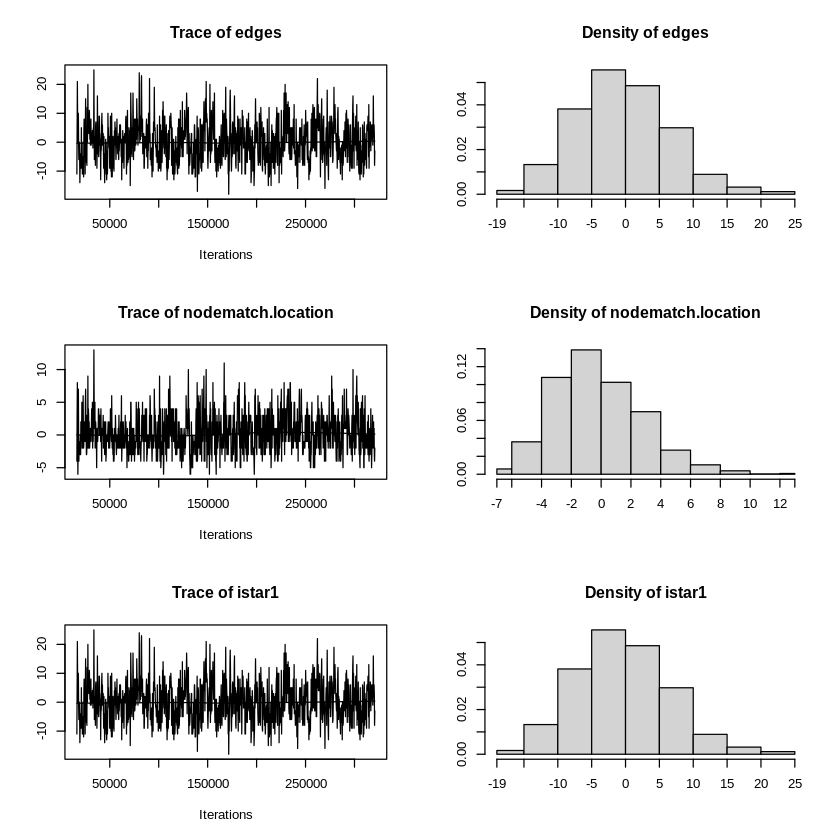
\includegraphics[scale=0.5]{images/ergm_diagnostics.png}
	\fautor
\end{figure}